\documentclass[letterpaper]{article}
\usepackage{amssymb}
\usepackage{fullpage}
\usepackage{amsmath}
\usepackage{epsfig,float,alltt}
\usepackage{psfrag,xr}
\usepackage[T1]{fontenc}
\usepackage{url}
\usepackage{pdfpages}
\usepackage{mathtools}
%\includepdfset{pagecommand=\thispagestyle{fancy}}
\author{Prof. Grizzle}
\title{Rob 501 - Mathematics for Robotics\\
HW \#6}

\begin{document}
\date{}
\maketitle


 \newcommand{\trace}{\mathrm{trace}}
\newcommand{\real}{\mathbb R}  % real numbers  {I\!\!R}
\newcommand{\nat}{\mathbb N}   % Natural numbers {I\!\!N}
\newcommand{\cp}{\mathbb C}    % complex numbers  {I\!\!\!\!C}
\newcommand{\ds}{\displaystyle}
\newcommand{\mf}[2]{\frac{\ds #1}{\ds #2}}
\newcommand{\Nagy}[2]{{Nagy, Page~#1, }{Prob.~#2}}
\newcommand{\spanof}[1]{\textrm{span} \{ #1 \}}
\newcommand{\argmin}{\arg\!\min}
\parindent 0pt


\begin{flushright}
{\bfseries Due Oct. 25, 2018 (Yes, no HW the week of Fall Break)} \\
{\bfseries 3PM via Gradescope}\footnote{Some of you still have not understood that GradeScope is purposely set to allow a 3 hour grace period. Hence, if you submit by 5:59 PM, you are fine; there is no late penalty. At 6:01 PM you are locked out. At 6:00 PM exactly, I have no idea what happens!} \\[3mm]
\end{flushright}



  \begin{itemize}
  \item{\textbf{Remark A)}}  There will be no HW due the week of Exam 1.

  \item{\textbf{Remark B)}} While the initial problems are on matrices, the main focus of this HW set is Recursive Least Squares (RLS), in other words, least squares estimation that can be implemented in a real-time environment. This is a good way to prepare for the Kalman Filter. The HW set looks long because lots of details are given for
each step in a problem, which should make the work go quickly.

  \item{\textbf{Remark C)}} To work the two problems on RLS, read the handouts \texttt{WeightedLeastSquares\_RLS.pdf}, which is typeset and the handout \texttt{RecursiveLeastSquares\_v02.pdf}, which is handwritten. They are basically the same, but the handwritten one has a bit more detail. Read the handout and then implement the algorithm. This may be a bit tough on you, but when we go through it in lecture, you will be remarkably well prepared. The hints give you a LOT OF INFORMATION. Read them!

  \end{itemize}


\begin{enumerate}


%Prob. 1 Matrices
\item The symmetric matrix below has distinct e-values.
Factor it as a product $O \Lambda O^\top$ where $O$ is an orthogonal matrix and $\Lambda$ is diagonal. It is OK to use MATLAB.
    $$A= \left[ \begin{array}{rrr} 2 &-1& 0 \\-1 &2 &1\\ 0& 1 &2 \end{array} \right]$$


%Prob. 2 Matrices
\item The symmetric matrix below has repeated e-values $2,2,-1$. In lecture, we stated that even with repeated e-values, we can still
diagonalize a symmetric matrix using orthogonal matrices. The objective of the problem is to see why this is true by working a numerical example. We will
 follow the proof attached at the end of the HW set and factor $A$ as a product $O \Lambda O^\top$, where $O$ is an orthogonal matrix.
    $$A=  \left[ \begin{array}{rrr} 1 &0& \sqrt{2} \\0 &2 &0\\ \sqrt{2} &0 &0\end{array} \right].$$
    Each of the steps below is motivated by a step in the proof. \textbf{Suggestion:} Open a script file in MATLAB and execute each step of the problem. It will save time.

        \begin{enumerate}
\setlength{\itemsep}{.1in}
\renewcommand{\labelenumi}{(\alph{enumi})}

\item  Verify that $v^1=[0, 1, 0]^\top$ satisfies $A  v^1 = 2 v^1$, and thus $v^1$ is an e-vector corresponding to $\lambda = 2$.

 \item Choose $v^2$ and $v^3$ such that $\{ v^1, v^2, v^3 \}$ is orthonormal, and verify that $V=[v^1~| v^2~| v^3 ]$ is an orthogonal matrix. In general,
 you would accomplish this by completing $\{v^1\}$ to a basis of $\real^n$ and applying Gram Schmidt. Here, you can do it by inspection.

 \item  Form the matrix $V^\top A V$ and verify that it has the form $$  \left[ \begin{array}{cc} 2 &0_{1\times2} \\ 0_{2 \times 1} &A_2 \end{array} \right]$$
 with $A_2$ symmetric.

 \item Use MATLAB to compute the e-values and e-vectors of $A_2$, and verify that they are $2,-1$, and thus distinct\footnote{If the e-values were repeated, you would find one e-vector, use it to build an orthonormal basis, and decompose $A_2$ to find $A_3$ symmetric that has dimension one less than $A_2$, etc.}. Find $U_2$ orthogonal such that
 $$U_2^\top A_2 U_2  $$
 is diagonal.  It is OK to use MATLAB for this.

 \item Define  the $3 \times 3$ matrix $U$ by
 $$ U =  \left[ \begin{array}{cc} 1 &0_{1\times 2} \\ 0_{2 \times 1} &U_2 \end{array} \right].$$
 Verify that $U$ is orthogonal.

 \item Define $O=V U$ and verify that $O$ is orthogonal.

 \item \textbf{This is the only part you turn in:} Report what you get when you compute $O^\top A O$. If it is not diagonal, you have done something wrong.

\end{enumerate}

%Prob. 3 Matrix Inversion Lemma
\item Write an \texttt{m-file} or \texttt{function} in MATLAB\footnote{It is OK to use a different programming language but please add enough comments that someone who does not know the language can still read it and see that it probably works.} that implements the Matrix Inversion Lemma
    $$ (A + BCD)^{-1} = A^{-1} - A^{-1}B(C^{-1} + DA^{-1}B)^{-1}DA^{-1}.$$
    Your function should assume that $A^{-1}$ is provided, that is, it should not compute the inverse of the matrix $A$, however it should compute the inverse of $C$. Verify that your function works by using the data in Prob. 4 of HW \# 5. \textbf{Turn in} your MATLAB code (print it out and insert it with your HW solutions).

%
%        $$A=\mathrm{diag}([1,~0.5, ~0.5,~1,~ 0.5]), ~ B=\begin{bmatrix} 1 \\ 0\\ 2\\ 0 \\3 \end{bmatrix}, C=0.2, D= B^\top $$
%

 %Prob. 4  Batch and recursive least squares
\item  Download the file \texttt{HW06\_Data.zip} from the CANVAS MATLAB folder and load the file \texttt{DataHW06\_Prob4.mat} into your MATLAB workspace (See also the ReadMe.txt file). The data file provides ``perturbed or noisy'' data for the model $y_i = C_i x + e_i$, $1 \le i \le N$, where $N=500$, $x\in \real^{100}$ and $y_i \in \real^3$. The data set contains the measured values $y_i$, the model matrices $C_i$, and the true value of $x$. The true value is given so that you can compare your estimated values to the true value. Of course, in real life, we would not have $x$ available to us. \\

For $1 \le k \le N$, define $S_k=I_{3 \times 3}$ and as in the lecture on Recursive Least Squares, $$ Y_k =\left[ \begin{array}{c} y_1 \\ \vdots \\ y_k \end{array} \right],~   A_k = \left[ \begin{array}{c} C_1 \\ \vdots \\ C_k  \end{array}  \right], ~ R_k = \mathrm{diag} [S_1, \cdots, S_k] = I.$$


\begin{enumerate}
\setlength{\itemsep}{.1in}
\renewcommand{\labelenumi}{(\alph{enumi})}

\item Find $n$ such that $A_k$ has at least $\mathrm{dim}(x)=100$  independent columns for $k\ge n$. For each $n \le k \le N$, define
$$ \hat{x}_k :=\mathrm{arg~min} ||Y_k - A_k x ||=\mathrm{arg~min} \sqrt{(Y_k - A_k x)^\top R_k(Y_k - A_k x)}$$
but do not compute anything except $n$ at this step.

\item For each $n \le k \le N$, compute $ \hat{x}_k $ in a batch process, that is,
$$  \hat{x}_k  = (A_k^\top R_kA_k)^{-1} A_k^\top R_k Y_k, $$
and, using the standard Euclidean norm, compute $$E_k :=||  \hat{x}_k  - x||.$$ Make a plot of $E_k$ versus $k$ and turn it in. Put a clear title on your plot, such as ``Norm error in x-hat using Batch Process''. Implementing the ``for each $n \le k \le N$'' will require a \texttt{for loop or while loop}. Use the \texttt{tic} and \texttt{toc} commands to determine how long it takes to compute your \textit{entire set of estimates} and report this value. Either write it on your error plot by hand or place it there with a MATLAB command.

\item For each $n \le k \le N$, compute $ \hat{x}_k $ using the RLS (Recursive Least Squares) Algorithm. First implement it without using the Matrix Inversion Lemma. Turn in a plot of $E_k$ versus $k$, and record on your plot the amount of time it takes to do your computations.

    \item For each $n \le k \le N$, compute $ \hat{x}_k $ once again using the RLS (Recursive Least Squares) Algorithm, but this time, implement it using the Matrix Inversion Lemma. Turn in a plot of $E_k$ versus $k$, and record on your plot the amount of time it takes to do your computations. Note that this time you are numerically inverting a $3 \times 3$ matrix and then computing the inverse of the $100 \times 100$ matrix $Q_k$ with the Matrix Inversion Lemma. This is the main point of the Matrix Inversion Lemma.

\end{enumerate}

%Prob. 5  Forgetting factor or exponential windowing
\item Download the file \texttt{HW06\_Data.zip} from the CANVAS MATLAB folder and load the file \texttt{DataHW06\_Prob5.mat} into your MATLAB workspace. It provides ``perturbed or noisy'' data for the model $y_i = C_i x_i + e_i$, $1 \le i \le N$, where this time the ``state'' or ``parameter'' $x$ that we are estimating is slowly ``drifting'' (means that it is slowly varying with time), which is why it has an index $x_i$. We will see that basic least squares does not work very well when $x$ can drift. We will learn a way to fix it.

   In this problem, $N=500$, $x\in \real^{20}$ and $y_i \in \real^3$. The data set contains the measured values $y_i$, the model matrices $C_i$, and the true value of $x_i$. The true value is given so that you can compare your estimated values to the true value. As you know very well, in real life, we would not have $x_i$ available to us. \\
    %%a \textit{forgetting} factor can be used to
\begin{enumerate}
\setlength{\itemsep}{.1in}
\renewcommand{\labelenumi}{(\alph{enumi})}

\item Find $n$ such that $A_k$ has at least $\mathrm{dim}(x)=20$  independent columns for $k\ge n$. For each $n \le k \le N$, define
$$ \hat{x}_k :=\mathrm{arg~min} ||Y_k - A_k x ||, $$
but do not compute anything except $n$ at this step. You should find $n=7$.

\item As in Prob. 4,  use constant weights, with $S_k = I_{3 \times 3}.$ For each $n \le k \le N$, compute $ \hat{x}_k $ (any method you wish)
and compute $E_k :=||  \hat{x}_k  - x_k||$. It does not matter how fast your MATLAB code is for the computation of $\hat{x}_k$ because in this problem we will not record the time. Make a plot of $E_k$ versus $k$ and turn it in. Put a clear title on your plot. Note that the error gets pretty bad.

\item \textbf{The forgetting factor:}  Let $0 < \lambda < 1$ (some number strictly between zero and one). A typical value for the \textit{forgetting factor} might be $\lambda = 0.98$. The idea is to discount old measurements when we do the least squares problem. This is done by selecting at time $k$ the weight matrices for $1 \le i \le k$  to be
    $$S_i= \lambda^{(k-i)}I_{3 \times 3}.$$ With this choice, the $3k \times 3k$  weighting matrix $R_k$ is given by
    $$R_k = \mathrm{diag} (\lambda^{k-1} I_3, \lambda^{k-2} I_3, \cdots, \lambda I_3, I_3).$$
    We see that the errors in older measurements are ``discounted''  by higher powers of $\lambda$, and thus the estimation process `` exponentially forgets'' them and  ``focuses'' on the more recent measurements.
It is important to note that at each step $k$, we are redefining the weights $R_k$ so that errors in the newest measurements are penalized the most. This can be done recursively in our \texttt{for loop}, by
    $$R_{k+1} = \left[ \begin{array}{cc} \lambda R_k & 0_{3k \times 3} \\ 0_{3 \times 3 k} & I_{3 \times 3} \end{array} \right].$$


For each $n \le k \le N$, compute $ \hat{x}_k $ using the Batch Method. Turn in a plot of $E_k$ versus $k$, and label your plot appropriately. You can use $\lambda = 0.98$ or you
can tune the forgetting factor to see what works best. How can you resist playing with it once you have your code working? :)

    \item For each $n \le k \le N$, compute $ \hat{x}_k $ now using the RLS (Recursive Least Squares) Algorithm, with forgetting factor. The algorithm (without using the Matrix Inversion Lemma) becomes
        \begin{itemize}
        \item \textbf{Initialization Step:} Set
        \begin{align*}
        Q_n:=&\sum_{i=1}^n C_i^\top \lambda^{n-i} C_i \\
        \Gamma_n:=&\sum_{i=1}^n C_i^\top \lambda^{n-i} y_i \\
        \hat{x}_n:=& (Q_n)^{-1} \Gamma_n
        \end{align*}


        \item \textbf{Recursion:} For $n \le k < N$
        \begin{align*}
        Q_{k+1}:=& \lambda Q_k + C_{k+1}^\top C_{k+1}\\
        K_{k+1}:= & (Q_{k+1})^{-1} C_{k+1}^\top \\
         \hat{x}_{k+1}:=&   \hat{x}_{k} + K_{k+1} \left( y_{k+1} - C_{k+1} \hat{x}_{k}  \right)
        \end{align*}

        \item If you want the version with the Matrix Inversion Lemma, see the hints!

        \item Turn in a plot of $E_k :=||  \hat{x}_k  - x_k||$ versus $k$, and label your plot appropriately.
        To be clear, there are no $\lambda$'s in the computation of $E_k$; we are just using the standard Euclidean norm to see how well we are doing in tracking
        $x$ as it slowly drifts.

         \end{itemize}
\end{enumerate}

% 10 Robotics Problem
\item  \textbf{Associating data to categories using distance:} Data association is a common task across various fields of Robotics. For example, if you have several pings from a sonar or radar, how do you know with which of several objects to associate them? You might enjoy the following YouTube video on the topic \url{https://www.youtube.com/watch?v=DK1DIcPwCOU}. \\

While doing data association, we look at the distance between a given point (or sample of data) and the mean (i.e. average value) of a finite set of possible categories, $S=\{S_1, S_2, \cdots, S_N\}$. The category assignment of a point $x$, called $C(x)$, is given by,
\begin{align}
C(x) = \argmin_{1 \le i \le N} ~ d (x, \mu_{S_i}),
\nonumber
\end{align}
where $\mu_{S_i}$ is the mean of category $S_i \in S$.
The most common distance used is the Euclidean distance,
\begin{align}
d_{Euc}(x, \mu_{S_i}) \coloneqq \vert\vert x - \mu_{S_i} \vert\vert_2
\nonumber
\end{align}
where $\mu_{S_1}$ is the mean of category $S_i$ and $\vert\vert x - \mu_{S_i} \vert\vert_2$ is the standard 2-norm.

While Euclidean distance works well as a coarse estimator, sometimes we have more information than just the mean of each category. One such form of information is the covariance matrix, which gives the uncertainty along every direction of set. A large value of covariance in a direction indicates a larger uncertainty along that direction. Conversely, a smaller covariance value indicates more confidence along that direction. \\ For example, consider a category $S_k$ with mean $\mu_{S_k} = \begin{bmatrix} 1 \\ 1 \\
\end{bmatrix} $ and covariance $\Sigma_{S_k} = \begin{bmatrix} 1 & 0 \\ 0 & 9 \\
\end{bmatrix}$. This can be represented as $S_{k} \sim N\left(\mu_{S_k}, \Sigma_{S_k}\right)$, the normal distribution with mean vector $\mu_{S_k}$ and covariance matrix $\Sigma_{S_k}$.
The covariance along the $x$-axis is $\Sigma_{S_k}^{11} = 1$, which indicates that the points in this category have $x$ values that are closer to the $\mu_{S_k}^x$ when compared to the $y$ values and  $\mu_{S_k}^y$ (since $\Sigma_{S_k}^{22} = 9$)

When the covariance matrix is available, we use a weighted 2-norm called the Mahalanobis distance. The Mahalanobis distance between a point and a category is defined as
\begin{align}
d_{M}(x, \mu_{S_i}) \coloneqq \vert\vert x - \mu_{S_i} \vert\vert_{\Sigma^{-1}} = \sqrt{(x-\mu_{S_i})^T\Sigma_{S_i}^{-1}(x-\mu_{S_i}) },
\nonumber
\end{align}
where $\mu_{S_1}$ is the mean and $\Sigma_{S_i}$ is the covariance matrix of category $i$ respectively. We recognize that we are using
$$<x,y>:= x^T\Sigma_{S_i}^{-1}y$$,
which gives the norm as $||x||=\sqrt{x^T\Sigma_{S_i}^{-1}x}$, as discussed in lecture.\\

Given 2 categories,
\begin{align}
S_1 \sim N\left({\begin{bmatrix} 4 \\ 0 \\
	\end{bmatrix},\begin{bmatrix} 0.25 & 0 \\ 0 & 2 \\
	\end{bmatrix}
}\right), ~~~ S_2 \sim N\left({\begin{bmatrix} 0 \\ 2 \\
\end{bmatrix},\begin{bmatrix} 6 & 2 \\ 2 & 2 \\
\end{bmatrix}
}\right)
\nonumber
\end{align}
Find the association of the following points using (a) Euclidean and (b) Mahalanobis distance
\begin{align}
(i)~P_1 =\begin{bmatrix} 4 \\ 2 \\    \end{bmatrix}
~~(ii)~P_2 = \begin{bmatrix} 2.8 \\ 1 \\    \end{bmatrix}
~~(iii)~P_3 =\begin{bmatrix} 2 \\ 0 \\    \end{bmatrix}
\nonumber
\end{align}
\begin{figure}[h]
		\centering
		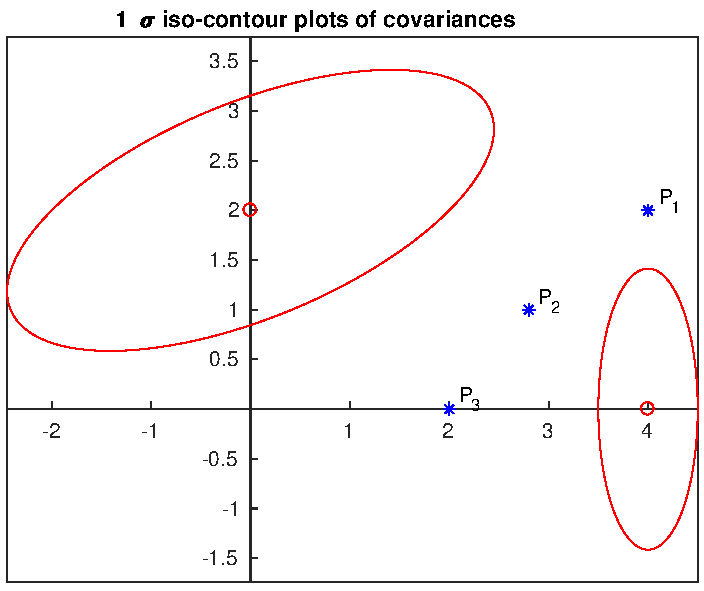
\includegraphics[width = 0.4\linewidth]{P6.pdf}
		\caption{Red ellipses are points that have $d_M = 1$ from means of $S_1$ and $S_2$ with corresponding covariances.}
\end{figure}

\textbf{Remark:} Note that the covariance matrices here are positive definite matrices. As mentioned above, we encountered this kind of matrix norm when we covered weighted least squares. The inverse of a Covariance matrix is called an Information matrix. We will be learning more about this when we do Kalman filters. (And a lot more in \textbf{EECS 568} - Mobile Robotics)

%End of list of HW Problems
\end{enumerate}

\newpage

\begin{center}
{\bf Hints}
\end{center}

\noindent \textbf{Hints: Prob. 2} The important point here is that when a matrix is symmetric, repeated e-values do not pose a problem as they do for a general square matrix.
The last page of the HW gives a proof by induction.

 \begin{enumerate}
\setlength{\itemsep}{.1in}
\renewcommand{\labelenumi}{(\alph{enumi})}

\item \textbf{Base Step:} The first thing to note is that a $1 \times 1$ matrix can always be factored.

\item \textbf{Inductive Step:} The induction hypothesis is to assume
that $(n-1) \times (n-1)$ symmetric matrices can be factored as $O \Lambda O^\top$ where $O$ is an orthogonal matrix and $\Lambda$ is diagonal.

\item \textbf{To show:} Next, you must show  that the same is true for
 $n \times n$ symmetric matrices. The key step in the proof is to show that if $A$ is symmetric and $\lambda$ is an e-value, then there exists an orthogonal matrix $P$ such
that
$$P^\top A P = \left[ \begin{array}{cc} \lambda  & 0_{1\times (n-1)} \\ 0_{(n-1) \times 1} & B \end{array} \right], $$
where $B$ is symmetric and $(n-1) \times (n-1)$. The orthogonal matrix $P$ is produced by using an e-vector associated with $\lambda$ and the Gram-Schmidt process. Hence, if you care
to understand the proof, it is within your means to do so.

\end{enumerate}

\vspace{1cm}

\noindent \textbf{Hints: Prob. 4 } Recursive Least Squares (RLS)

  \begin{enumerate}
\setlength{\itemsep}{.1in}
\renewcommand{\labelenumi}{(\alph{enumi})}

\item \textbf{Basic Version:}

         \begin{itemize}
        \item \underline{Initialization Step:} Choose $n$ such that $Q_n$ is invertible (full rank)
        \begin{align*}
        Q_n:=&\sum_{i=1}^n C_i^\top S_i C_i \\
        \Gamma_n:=&\sum_{i=1}^n C_i^\top S_i y_i \\
        \hat{x}_n:=& (Q_n)^{-1} \Gamma_n
        \end{align*}


        \item \underline{Recursion:} For $n \le k < N$
        \begin{align*}
        Q_{k+1}:=& Q_k + C_{k+1}^\top S_{k+1}C_{k+1}\\
        K_{k+1}:= & (Q_{k+1})^{-1} C_{k+1}^\top S_{k+1} \\
         \hat{x}_{k+1}:=&   \hat{x}_{k} + K_{k+1} \left( y_{k+1} - C_{k+1} \hat{x}_{k}  \right)
        \end{align*}

         \end{itemize}

        \item  \textbf{Improved Version Using the Matrix Inversion Lemma:}
 \begin{itemize}


        \item \underline{Initialization Step:} Choose $n$ such that $Q_n$ is invertible (full rank)
        \begin{align*}
        Q_n:=&\sum_{i=1}^n C_i^\top S_i C_i \\
        P_n:= &(Q_n)^{-1} \\
        \Gamma_n:=&\sum_{i=1}^n C_i^\top S_i y_i \\
        \hat{x}_n:=& P_n \Gamma_n
        \end{align*}

        \item \underline{Recursion:} For $n \le k < N$
        \begin{align*}
         P_{k+1}  =&  P_k -  P_k C_{k+1}^\top [ S_{k+1}^{-1} +  C_{k+1}  P_k  C_{k+1}^\top ]^{-1}C_{k+1} P_k.\\
        K_{k+1}:= & P_{k+1} C_{k+1}^\top S_{k+1} \\
         \hat{x}_{k+1}:=&   \hat{x}_{k} + K_{k+1} \left( y_{k+1} - C_{k+1} \hat{x}_{k}  \right)
        \end{align*}

        \item \underline{How to Derive the Riccati Equation? It comes from the Matrix Inversion Lemma}

\begin{align*}
Q_{k+1}  = & Q_k + C_{k+1}^\top S_{k+1} C_{k+1} \\
  Q_{k+1}^{-1} = & \left( Q_{k} + C_{k+1}^\top S_{k+1} C_{k+1}\right)^{-1} \\
   =& Q_k^{-1} -  Q_k^{-1}C_{k+1}^\top \left[ S_{k+1}^{-1}  + C_{k+1}  Q_k^{-1}  C_{k+1}^\top \right]^{-1} C_{k+1} Q_k^{-1}\\
   P_k:=  &Q_k^{-1}\\
   P_{k+1}  =&  P_k -  P_k C_{k+1}^\top \left[ S_{k+1}^{-1} +  C_{k+1}  P_k  C_{k+1}^\top \right]^{-1}C_{k+1} P_k.\\
    \end{align*}

    \item Jacopo Francesco Riccati (1676-1754) \url{http://en.wikipedia.org/wiki/Jacopo_Riccati}

           \end{itemize}

         \end{enumerate}
\vspace{1cm}

\noindent \textbf{Hints: Prob. 5 }
 \begin{enumerate}
\setlength{\itemsep}{.1in}
\renewcommand{\labelenumi}{(\alph{enumi})}

\item Rewrite $ Q_{k+1} = \lambda Q_k + C_{k+1}^\top C_{k+1}$ as
$$ \frac{1}{\lambda} Q_{k+1} = Q_k + C_{k+1}^\top \frac{1}{\lambda}  C_{k+1}$$
Therefore
$$ {\lambda} Q_{k+1} ^{-1} = [Q_k + C_{k+1}^\top \frac{1}{\lambda}  C_{k+1}]^{-1}~~~(*)$$
Using the Matrix Inversion Lemma, we have
$$ {\lambda}Q_{k+1}^{-1} = Q_k^{-1} -  Q_k^{-1}C_{k+1}^\top [\lambda I +  C_{k+1}  Q_k^{-1}  C_{k+1}^\top ]^{-1} C_{k+1} Q_k^{-1}.$$
and thus
$$ Q_{k+1} ^{-1} = \frac{1}{\lambda}  Q_k^{-1} -  \frac{1}{\lambda}  Q_k^{-1}C_{k+1}^\top [\lambda I +  C_{k+1}  Q_k^{-1}  C_{k+1}^\top ]^{-1} C_{k+1} Q_k^{-1}.$$
If we define $P_k:=Q_k^{-1}$, we obtain
$$ P_{k+1}  = \frac{1}{\lambda}  P_k -  \frac{1}{\lambda}  P_k C_{k+1}^\top [\lambda I +  C_{k+1}  P_k  C_{k+1}^\top ]^{-1} C_{k+1} P_k.$$
\item If you are using your m-file for the Matrix Inversion Lemma, you can stop at (*), apply your function to get the inverse of $ [Q_k + C_{k+1}^\top \frac{1}{\lambda}  C_{k+1}]$, and
then divide by the forgetting factor.

\item The recursion on $\hat{x}_k$ is unchanged from the RLS algorithm without the forgetting factor. In case you want to see the derivation, the key formulas are:
    \begin{align*}
    Q_k := &\sum_{i=1}^k C_i^\top \lambda^{k-i} C_i \\
Q_k \hat{x}_k :=&\sum_{i=1}^k C_i^\top \lambda^{k-i} y_i \\
Q_{k+1}  = &\sum_{i=1}^{k+1} C_i^\top \lambda^{k+1-i} C_i \\
 =& \lambda Q_k + C_{k+1}^\top C_{k+1} \\
 Q_{k+1} \hat{x}_{k+1} =&\sum_{i=1}^{k+1} C_i^\top \lambda^{k+1-i} y_i \\
 = & \lambda \sum_{i=1}^k C_i^\top \lambda^{k-i} y_i + C_{k+1}^\top y_{k+1} \\
 =& \lambda Q_k \hat{x}_k +  C_{k+1}^\top y_{k+1}     \\
  \lambda Q_k = & Q_{k+1} - C_{k+1}^\top C_{k+1}
    \end{align*}
    and thus, putting all of this together
    \begin{align*}
    \hat{x}_{k+1} = & Q_{k+1}^{-1} \left[ \left( Q_{k+1} - C_{k+1}^\top C_{k+1} \right) \hat{x}_k + C_{k+1}^\top y_{k+1} \right] \\
 =  &\hat{x}_k + Q_{k+1}^{-1} C_{k+1}^\top \left( y_{k+1} - C_{k+1} \hat{x}_k \right)
    \end{align*}
    Hence, the only change is to the update formula for $Q_{k+1}$.

\end{enumerate}

\newpage
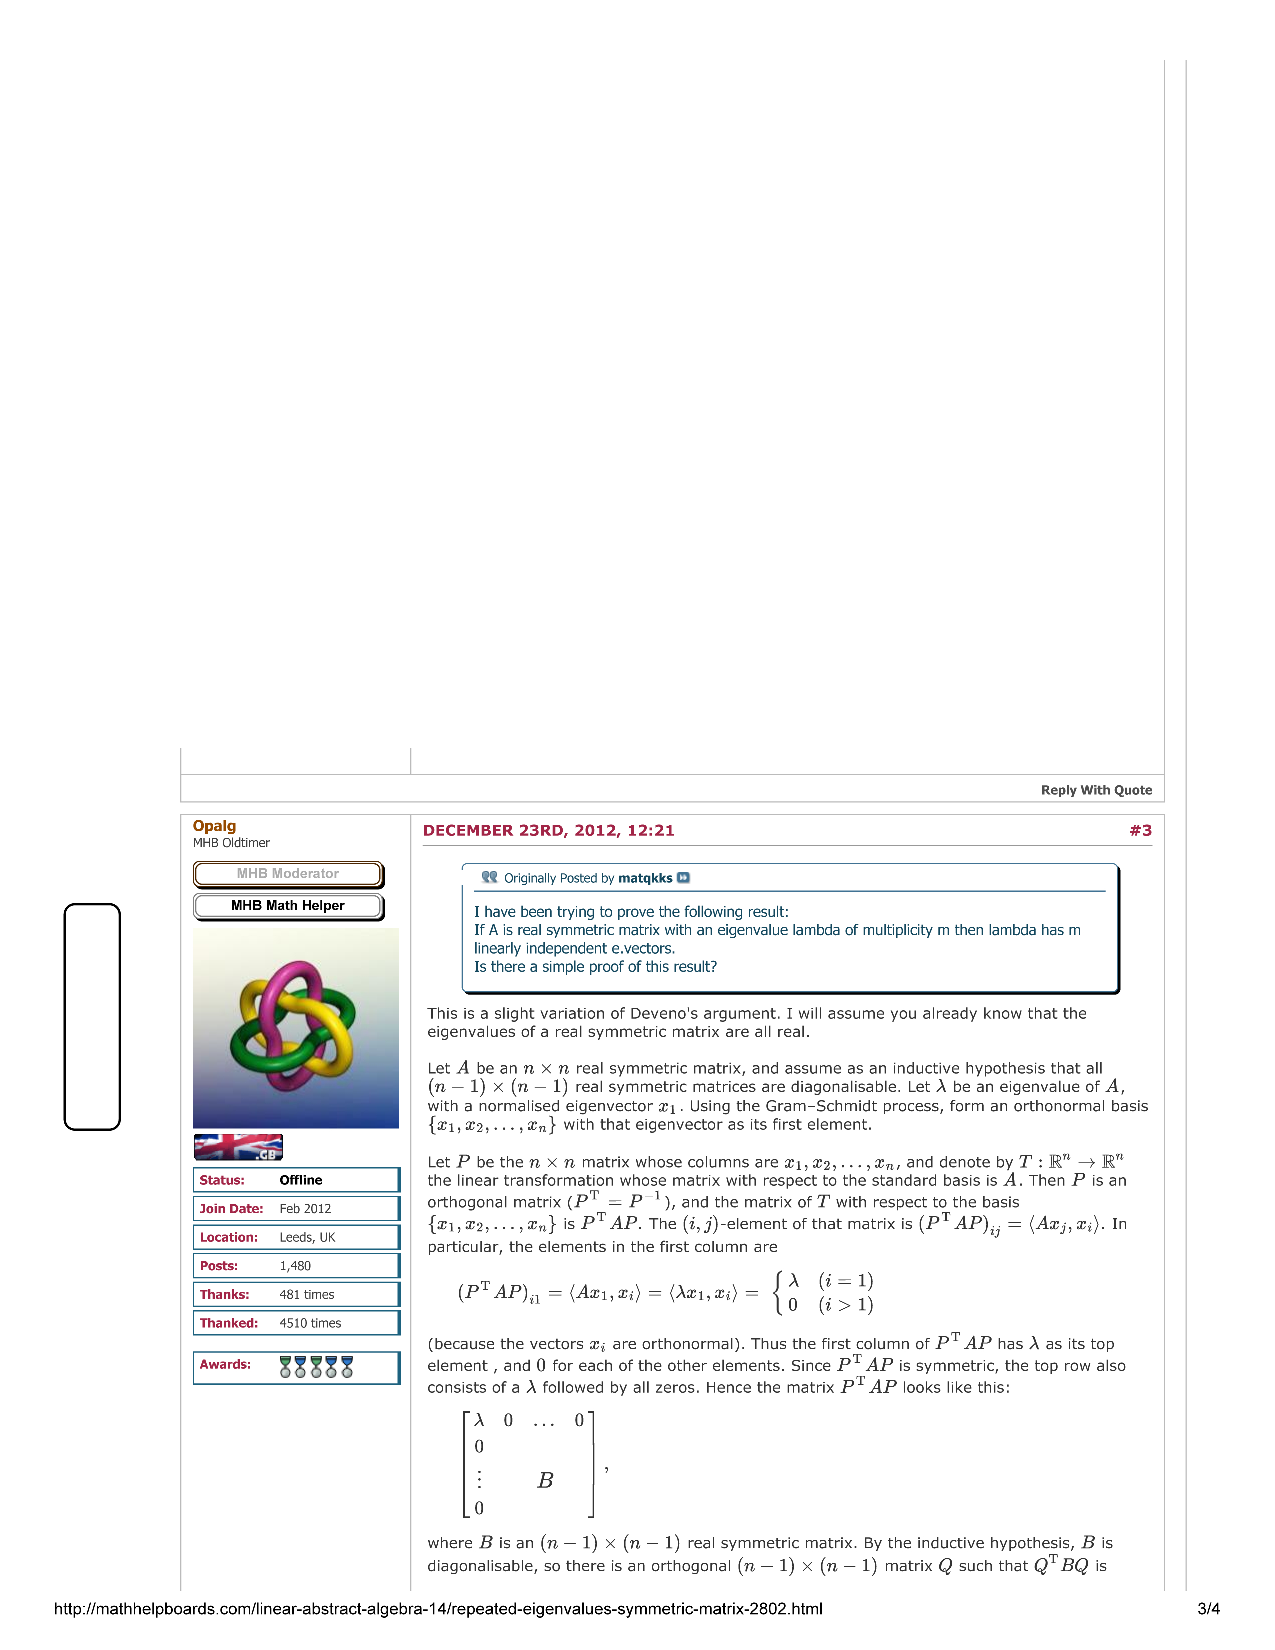
\includepdf[pages=-]{LinearAlgebraSymmetricRepeatedEigenvaluesInductionProof.pdf}


\end{document}


